\documentclass[a4paper,11pt]{article}
\usepackage{graphicx}
\title{Software Requirements Specification \\ Bin-packing VM Consolidation Algorithm}
\author{Atchutuni Bhavana \\ Terli Venkatesh \\ Surineni Sampath Kumar}
\date{\today}

\begin{document}
	\maketitle
	 \pagebreak 
	 \tableofcontents
	 \pagebreak 

	\section{INTRODUCTION}
		\subsection{Product overview}
		This project takes as  input 
		\begin{itemize}
		  \item Physical machines and their capacities
		  \item Virtual machines and their capacity requirements
		  
		\end{itemize} 
		It computes the residual capacity in each physical machine after adding the 
		virtual machines. The physical machines are sorted in ascending order of their residual capacity. 
		The project provides the feature of consolidating the virtual machines in different physical machines into 
		minimum number of physical machines. Another feature provided by this project is to shutdown a physical system
		by migrating the virtual machines in that physical machine into other physical machines. This project uses
		greedy bin packing algorithm for this purpose. \section{SPECIFIC REQUIREMENTS}
		\subsection{External Interface Requirements}
			\subsubsection{User Interfaces}
			
			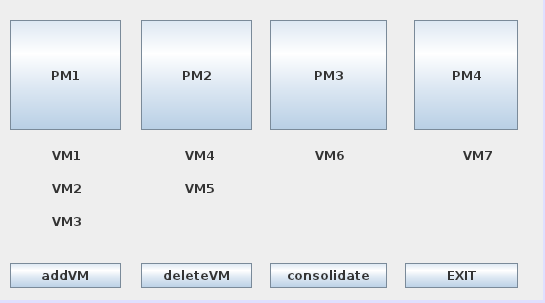
\includegraphics[height=10cm]{images/gui}
			\\
			\\
			The GUI displays 			
			\begin{itemize}
				\item All the physical machines
				\item Virtual Machines in each physical machine
				\item Buttons for adding a vm, deleting a vm, for consolidation and turning off 
				the physical machine
			\end{itemize}

			\subsubsection{Hardware Interfaces}
			No specific hardware module is being used for this project
			\subsubsection{Software Interfaces}
			No specific software module is being used for this project 
			\subsubsection{Communication Protocols}
			This project doesn’t use any communication protocols
		\subsection{Software Product Features}
			\begin{enumerate}
				\item {\bf Provides the ability to add a vm} \\
				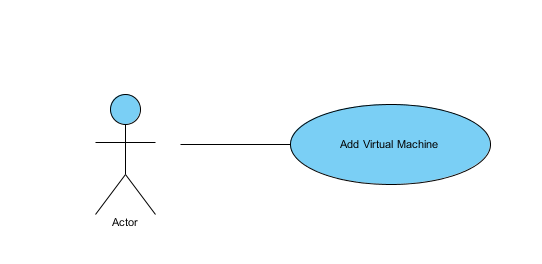
\includegraphics{images/usecase}
				\\This action is triggered by user clicking {\bf Add VM } Button. A new window appears with fields for  
				\begin{itemize}
				 \item Capacity of the VM
				 \item VM ID to be given to the VM
				\end{itemize}
				
				This would return \\
				{\bf On Success: }\\
				The GUI will be updated showing that new  VM that is added to existing PM.
				The residual capacity of the PM is calculated and updated to reflect in GUI\\\\
				{\bf On Failure: } \\
				{\bf Reason: No enough residual capacity to accomodate a VM}\\
				The user will get an error message that there is no enough space to add the given VM\\
				{\bf Reason: User has chosen a PM that is switched off}\\
				The user will get an error message that the selected PM is switched off
				\item {\bf Provides the ability to delete a vm}\\
				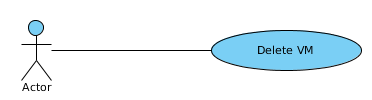
\includegraphics{images/delete}
				\\This action is triggered by user clicking {\bf Delete VM } Button. A new window appears with fields for  
				\begin{itemize}
				 \item Choosing the PM in which the VM we want to delete resides. Then a drop down list will be
				 updated with list of VM's in the chosen PM.
				 \item The user has to select the  ID of the VM that we want to delete from the drop down list. Only VM's that are alive will be displayed in the list.
				\end{itemize}
				
				This would return \\
				{\bf On Success: }\\
				The GUI will be updated showing that new  VM that is deleted from the PM.
				The residual capacity of the PM is calculated and update to reflect in GUI\\\\
				{\bf On Failure: } \\
				{\bf Reason: The selected PM is empty or switched off}\\
				The user will get an error message that the particular PM which you have selected is empty or 
				switched off
				
				%\item Displays the details of which vm is in which pm
				
				
				\item {\bf Ability to switch off a physical machine}\\
				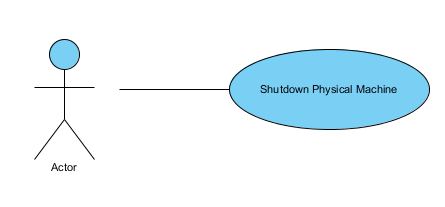
\includegraphics{images/shut}
				\\This action is triggered by user clicking on the PM which he wants to shutdown. 
								
				This would result in \\\\
				{\bf On Success: }\\
				The software moves all the VM's into other PM's with sufficient residual capacity. Then the system is shutdown. 
				The GUI will be updated showing that the PM selected is switched off
				\\\\
				{\bf On Failure: } \\
				{\bf Reason: VM's in the selected PM cannot be accomodated in other PM's}\\
				The user will get a message stating that the VM's in the selected PM cannot be accomodated in other PM's.
				
				\item {\bf Ability to switch on a physical machine}\\
				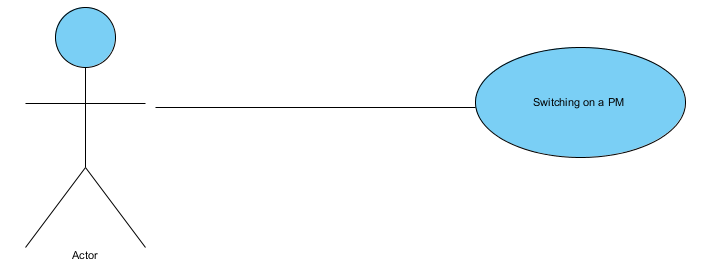
\includegraphics[scale=0.7]{images/onpm}
				\\This action is triggered by user clicking on the PM which he wants to switch on. 
				
				This would result in \\\\
				{\bf On Success: }\\
				The PM will be switched on. The color of the PM is changed from red to green to reflect the on 
				status of PM in GUI 
				
				
				
				\item {\bf Provides the ability to consolidate all VM's in minimum number of PM's}\\
				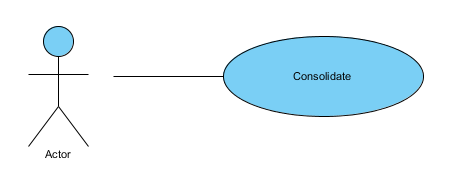
\includegraphics{images/consolidate}
 				\\This action is fired by user clicking the {\bf consolidate} Button. 
								
				This would result in \\\\
				{\bf On Success: }\\
				The software runs Bin packing algorithm. Moves the VMs into as few PMs as possible. Updates the GUI
				\\
				

			\end{enumerate}
			
			
			
			
			
			
%	\section{SOFTWARE SYSTEM ATTRIBUTES}
%
%	  {\bf Performance}
%	  \\	  
%	  
%	    Performance is an indication of the responsiveness of a system to execute any action within a 
%	    given time interval. It can be measured in terms of latency or throughput. Latency is the time 
%	    taken to respond to any event. Throughput is the number of events that take place within a given amount of time.
%	    \\\\	    
%	 {\bf Reliability}
%	 \\
%	  
%	    Reliability is the ability of a system to remain operational over time. Reliability is measured as 
%	    the probability that a system will not fail to perform its intended functions over a specified time interval.
%	    \\\\	
%	  {\bf Availability}
%	  \\
%	  
%	    Availability defines the proportion of time that the system is functional and working. It can be measured 
%	    as a percentage of the total system downtime over a predefined period. Availability will be affected by 
%	    system errors, infrastructure problems, malicious attacks, and system load.
%	    \\\\
%	  {\bf Security}
%	  \\
%	  
%	    Security is the capability of a system to prevent malicious or accidental actions outside of the designed 
%	    usage, and to prevent disclosure or loss of information. A secure system aims to protect assets and prevent 
%	    unauthorized modification of information.
%	    \\\\\\\\
%	  {\bf Maintainability}
%	  \\
%	  
%	    Maintainability is the ability of the system to undergo changes with a degree of ease. These changes could 
%	    impact components, services, features, and interfaces when adding or changing the functionality, fixing 
%	    errors, and meeting new business requirements.
%	    \\\\
%	  {\bf Portability}
%	  \\
%	  
%	    Portability in high-level computer programming is the usability of the same software in different environments. 
%	    The prerequirement for portability is the generalized abstraction between the application logic and system 
%	    interfaces. When software with the same functionality is produced for several computing platforms, portability
%	    is the key issue for development cost reduction.
%
%

\end{document}
